% !TEX encoding = UTF-8 Unicode
\documentclass[a4paper,12pt,italian,twoside]{book}   	% use "amsart" instead of "article" for AMSLaTeX format
%\usepackage[parfill]{parskip}    		% Activate to begin paragraphs with an empty line rather than an indent
\usepackage{graphicx}				% Use pdf, png, jpg, or epsß with pdflatex; use eps in DVI mode
								% TeX will automatically convert eps --> pdf in pdflatex		
\usepackage{amssymb}
\usepackage[italian]{babel}			% Traduce in italiano tutte le parti
\usepackage[utf8]{inputenc}			% Permette l'inserimento di caratteri in UTF-8

\usepackage{hyperref}				% Per rendere cliccabile l'indice
\hypersetup{colorlinks=true,linkcolor=blue}

%\setcounter{tocdepth}{1}			% Setta la profondità dell'indice

\title{Un titolo fantasioso}
\author{Andrea Peretti}
\date{\today}							% Activate to display a given date or no date

\includeonly{cap1}

\begin{document}

\maketitle
\tableofcontents

%%%%%%%%
% !TEX encoding = UTF-8 Unicode

\chapter{Introduzione}
L'informatica è il settore tecnologico che si evolve con maggiore velocità. La Prima legge di Moore\footnote{La prima legge di Moore è un'osservazione empirica di Gordon Moore, cofondatore di \emph{Fairchild Semiconductor} e di \emph{Intel}.} asserisce che la potenza dei calcolatori raddoppia ogni diciotto mesi. Una simile progressione in un settore tecnologico assai più anziano come l'aeronautica, permetterebbe oggi di fare un giro completo della terra in una manciata di secondi. Questa potenza di calcolo permette lo sviluppo di applicazioni impensabili fino ad una decina di anni fa, capaci di trattare una quantità di dati da elaborare estremamente grande. Un esempio significativo è l'ammontare di dati che viene generato dai sensori dell'acceleratore di particelle del CERN di Ginevra\footnote{\cite{pres_cern}}, sono circa 15 PetaByte l'anno, i quali devono essere memorizzati e poi elaborati. Il web tutt'oggi genera dati analoghi, ed ogni giorno vengono memorizzati diversi terabyte di dati a seguito di ricerche, acquisti, pubblicazione di contenuti sui social network, eccetera. 
\begin{figure}
	\centering
	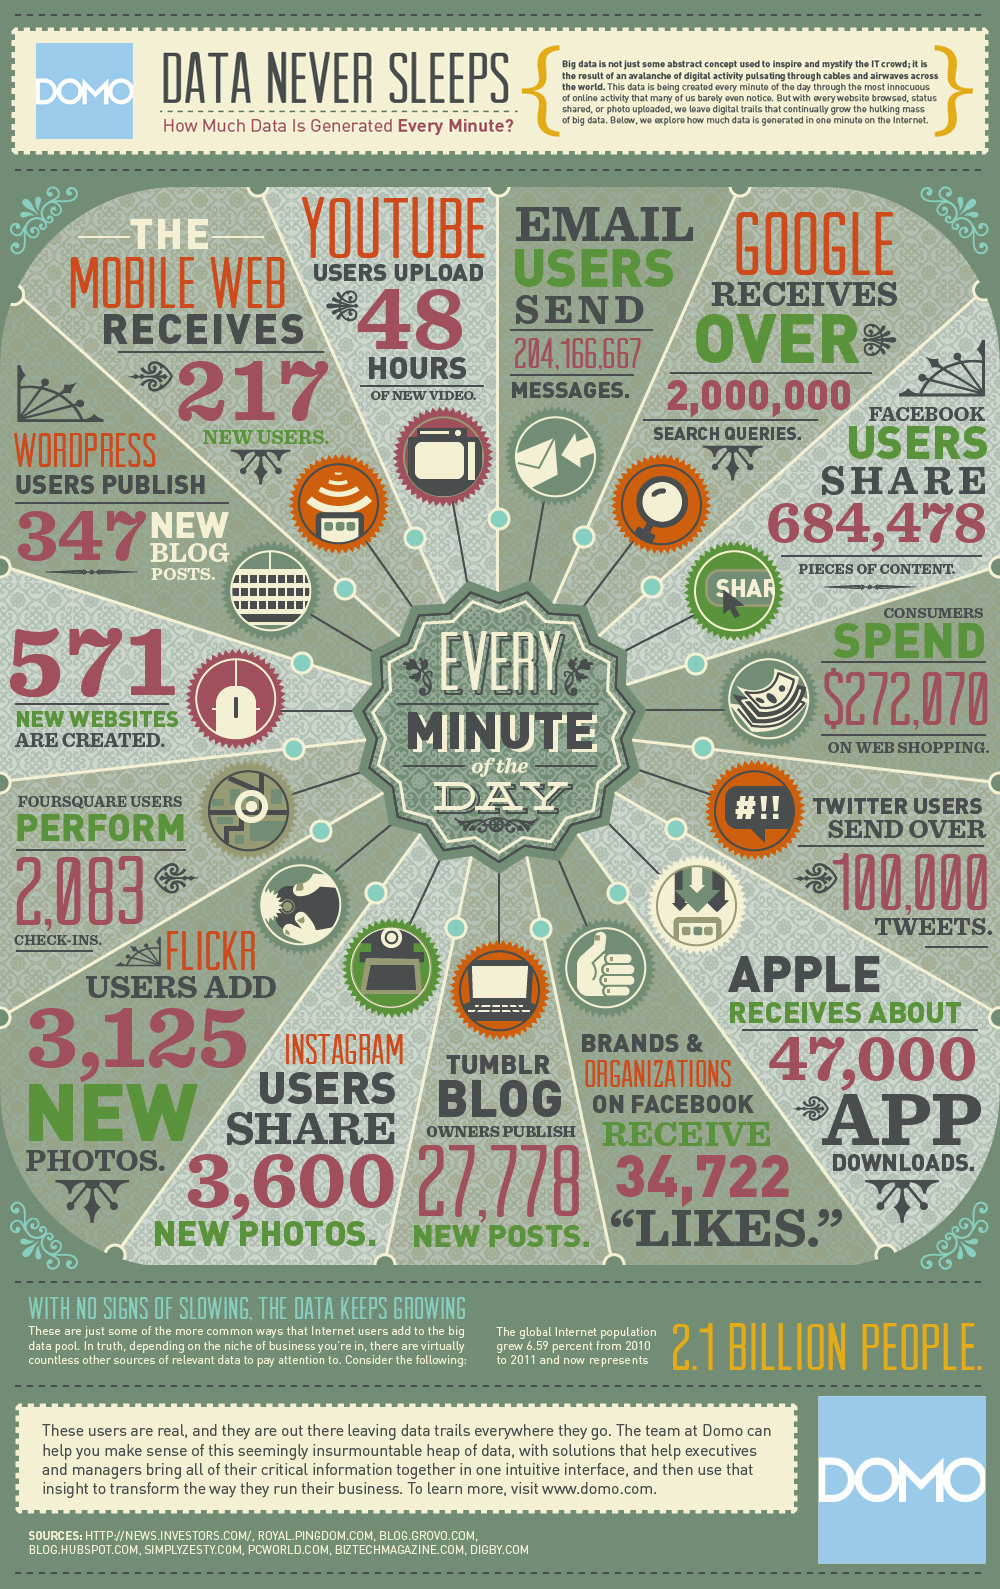
\includegraphics[width=0.50\textwidth]{Data-in-One-Minute.jpg}
	\caption{Quantità di dati al minuto generati dagli utenti di alcuni siti in rete.}
	\label{img:dpm}
\end{figure}
L'infografica nella figura \ref{img:dpm}\footnote{\cite{data_per_minute}} ci permette di vedere con immediatezza di quali quantità stiamo parlando, e possiamo evincere che per una tale mole di informazioni occorrono delle procedure di trattamento dell'informazione diverse da quelle che possono essere adottate da un programma per gestire una semplice rubrica. Stiamo parlando quindi di diversi GigaByte se non TeraByte di dati, che hanno bisogno di essere analizzati e processati in tempo modesto. I tipi di elaborazione necessari possono essere il calcolo di statistiche, una suddivisione per categoria, un'interrogazione della base di dati, oppure una serie di calcoli che possono permettere ad un'azienda di capire, in base agli acquisti dei suoi clienti, i trend riguardo i suoi prodotti. Le tecniche elaborate nel corso degli anni hanno portato alla nascita di una nuova branca dell'informatica, quella dei \emph{Big Data}. Con questo termine non si intendono solo i dataset di grandi dimensioni, ma anche le tecniche utilizzate per \emph{elaborarli} ed estrarre informazioni significative da esso. Spesso non è vero che i dati di un dataset siano omogenei e che tutti rispettino la stessa struttura, perché possono essere il risultato dell'unione di più basi di dati, l'aggiunta di nuovi record può essere effettuata da entità diverse le quali non si preoccupano di seguire una forma standard, per questo motivo è necessario che siano prima \emph{elaborati}. L'\emph{obbiettivo} di queste tecniche è quindi quello di estrarre \emph{informazioni significative}, per le quali intendiamo qualsiasi tipo di statistica che possa essere calcolata solamente prendendo in considerazione tutti i dati esistenti, impossibile da calcolare a mano o farsene un'idea "guardando" i dati. Tornando alla figura \ref{img:dpm}, il risultato dell'elaborazione dei dati è stato presentato in modo da avere un chiaro riscontro, dando la possibilità al lettore di trarre immediatamente le proprie conclusioni sulla globalità dei dati.
Si può suddividere il processo che vede entrare in gioco i big data in tre parti:
\begin{enumerate}
\item Raccolta dei dati
\item Elaborazione
\item Visualizzazione
\end{enumerate}
La raccolta dei dati è la prima parte del processo, e tratta la memorizzazione dei dati ed il loro mantenimento. Non è detto che memorizzazione avvenga su database, ma in qualunque modo, come file di testo o fogli elettronici. Spesso però questa fase è effettuata per altri scopi piuttosto che per effettuare delle elaborazioni tramite gli strumenti dei Big Data. Questo può comportare un dataset formato da dati provenienti da fonti diverse, che utilizzano tecnologie e standard diversi che devono essere aggregati, inoltre non tutti i record potrebbero essere completi, con campi mancanti, dati non consistenti eccetera. Anche questi problemi dovranno essere affrontati.
La parte di elaborazione prevede una serie di tecniche atte ad analizzare tutti i dati in un tempo accettabile, ed effettuare i calcoli. Questa parte prevede anche tutti quegli algoritmi statistici utili ad estrarre informazioni significative da campioni di dati.
La parte di visualizzazione si occupa di presentare i risultati in modo che sia possibile interpretarli immediatamente e farsi un'idea delle proprietà emerse dall'elaborazione rispetto alla totalità dei dati.
In questo testo verranno accennate le prime due parti, mentre per terza parte si presenteranno strumenti di programmazione utili allo scopo, per essere poi applicati al progetto \emph{Piedmont Heritage}.

%%%%%%%%
% !TEX encoding = UTF-8 Unicode
\chapter{Concetti}%Decidere se trasformare in un capitolo di teoria, in cui si parla anche del pattern MVC

\section{Big Data}\label{sec:bigdata}
Secondo \cite{rezzani2013big} i Big Data
\begin{quotation}
sono dati che superano i limiti degli strumenti di database tradizionali.
\end{quotation} 
		
\subsection{Acquisizione}
\subsection{Elaborazione}
\subsection{Visualizzazione}
\section{Modello Client/server}%Veramente serve??
\section{Pattern MVC}
\subsection{Model}
\subsection{View}
\subsection{Controller}
	
	

%%%%%%%%
% !TEX encoding = UTF-8 Unicode
\chapter{Analisi del progetto}
	\section{Descrizione}
	\emph{Piedmont Heritage} è il progetto finale sviluppato durante il corso \emph{Big Dive 2}\footnote{Il sito di Big Dive è \url{http://www.bigdive.eu}} dal sottoscritto insieme con \emph{Maximilien Rzepka} e \emph{Marco Sors}. \`{E} possibile visualizzare il progetto online all'indirizzo \url{http://piedmontheritage.bigdive.eu}, la cui versione è attualmente quella precedente alle modifiche descritte in questo testo.
	
	Il sito mostra una serie di "slide" in cui vengono visualizzate informazioni su locali ed oggetti storici presenti in Piemonte. Partendo dall'alto è presente una mappa che visualizza l'ubicazione dei locali ed a seguire una serie di infografiche rappresentanti le categorie dei locali presenti, il periodo in cui sono nati, ed infine un grafico sulle tipologie di oggetti, il inframmezzato da citazioni e detti popolari inerenti a Torino ed al Piemonte.
	
	\section{Contesto in cui il progetto è stato realizzato}
	Piedmont Heritage è stato sviluppato nell'ultima settimana di Big Dive, come prova finale in cui si sarebbero utilizzati tutti i concetti e gli strumenti presentati durante il corso. Dal sito del corso, \begin{quote}
	BIG DIVE è un programma di formazione volto a promuovere una nuova generazione di sviluppatori.
	Una palestra combattimento da strada, dove dataset di alto valore sono la materia prima nelle mani di un gruppo di appassionati seguiti da esperti in tre aree chiave: 
	Development, Data Science and Visualization.
	\end{quote}
	La nascita di questo progetto è stata dettata dallo spirito del corso: scegliere dei compagni di lavoro, scegliere un dataset tra quelli messi a disposizione, capire che cosa offre il dataset ed elaborare dei dati da esso, utilizzando la creatività del gruppo.
	
	Durante il corso sono stati affrontati argomenti inerenti ai Big Data, dal calcolo di statistiche basate sulle basi di dati alla visualizzazione di quest'ultime in modo \emph{bello}, \emph{immediato} ed \emph{esaustivo}. Sarà quest'ultima parte l'argomento di questo testo, dove si affrontaterà il problema di \emph{come visualizzare i dati su una mappa}.
	
	\section{Il dataset}
	Il dataset utilizzato è il \textbf{Guarini Dataset}, il quale è un progetto della Regione Piemonte nato ai fini di \begin{quote}%??Visualizzare il link?? ??Utilizzare quotation?? 
	migliorare la definizione dei programmi di intervento, salvaguardia e valorizzazione.\footnote{Tratto dal sito ufficiale della Regione: \url{http://www.regione.piemonte.it/cultura/guarinipat/index.htm}}
	\end{quote}%Il dataset ci è stato fornito come due file di foglio elettronico, contenenti rispettivamente i locali e gli oggetti.
	Il Sistema Informativo Guarini è il software fornito dalla Regione Piemonte utilizzato per il censimento sancito dall'art. 2 della L.R. 34/95\footnote{\url{http://arianna.consiglioregionale.piemonte.it/base/leggi/l1995034.html}} e L.R 35/95\footnote{\url{http://arianna.consiglioregionale.piemonte.it/base/leggi/l1995035.html}}. I locali storici presenti nel dataset sono selezionati dai consigli comunali appartenenti al luogo in cui si trovano, e vengono censiti solo se meritevoli. L'aggiunta dei dati al dataset è caratterizzata da una grande libertà nel tipo di informazioni inseribili, inoltre ogni record è inserito da persone diverse, con la conseguenza di una frammentazione dei dati presenti nel database, con campi non compilati e campi ad-hoc per alcune entry.
	\subsection{Una nota a proposito del database}
	Anche se il corso tratta i \emph{Big Data} il dataset è molto ristretto, conta infatti circa 1200 entry, che dopo essere state selezionate e corrette sono scese a circa 900. Alla fine del corso per questo motivo il progetto non era ottimizzato nel caso in cui il numero di entry fosse aumentato, cosa a cui si è provveduto successivamente a scopo didattico. Inoltre, con un numero così basso di elementi non è stato necessario utilizzare i metodi studiati per l'elaborazione di grandi moli di dati visti nel corso, per questo motivo nei prossimi capitoli se ne accennerà solamente.
	
	
	\section{La mappa}
	La parte che verrà analizzata è quella della prima slide, la \emph{mappa dei locali}. Durante lo sviluppo l'obbiettivo è stato trovare ed utilizzare uno strumento che permettesse di \emph{visualizzare dei segnalini} su di una mappa in corrispondenza dei locali memorizzati nel dataset, \emph{filtrare} quali risultati visualizzare e mostrare i \emph{dettagli del locale} il cui segnalino è stato cliccato.
	Per farlo sono stati utilizzati alcuni strumenti presentati nel corso, mentre altri sono stati scelti liberamente.
	\subsection{Miglioramenti dopo Big Dive}
	Durante l'A.A. successivo a quello dello stage, sono stati effettuati dei miglioramenti alla mappa della prima slide di Piedmont Heritage da parte dell'autore, permettendo una maggiore libertà per il filtraggio dei risultati, migliorando la navigazione tra di essi, implementando un sistema per ottenere dati dal server in modo asincrono con il caricamento della pagina e risolvendo un bug.
	Il sito inoltre è ora servito tramite un framework presentato durante lo stage: queste modifiche sono state effettuate per rendere il progetto utilizzabile per basi di dati più grosse, come descritto nei prossimi capitoli, ma anche a scopo didattico in modo da utilizzare altri strumenti presentati nel corso.

%%%%%%%%
% !TEX encoding = UTF-8 Unicode
\chapter{Strumenti utilizzati}
Nella realizzazione del progetto sono stati affrontati molti problemi, in alcuni casi adottando soluzioni comuni nel mondo della programmazione online\footnote{Ad esempio nella manipolazione del DOM, è stata utilizzata una libreria JavaScript chiamata JQuery}, altre realizzate in modo specifico per il progetto. Le problematiche affrontate, tenendo conto delle richieste dei fornitori del dataset, sono state quelle di mostrare i dati nel modo più esplicativo possibile senza fornire la possibilità di accedere direttamente al dataset, utilizzando solo l'interfaccia front-end sviluppata. Il programma quindi effettua delle richieste asincrone al server per ottenere alcune parti del dataset, formattate in modo da contenere solo i dati necessari alla visualizzazione corretta sulla mappa dei punti di interesse.

Un altri obbiettivi da raggiungere sono stati:
\begin{itemize}
	\item Rendere possibile una crescita del progetto in futuro

Il progetto è stato strutturato in modo da rendere possibile in futuro l'aggiunta di funzioni ed aggiungere nuovi locali, tenendo ben presente che i pochi record attuali sono molto semplici da gestire, mentre se dovessero aumentare di molto il programma è comunque capace di gestire i nuovi record senza appesantirsi di un overhead troppo elevato.

	\item Utilizzare un database

Siccome il dataset iniziale era un semplice file CSV che necessitava di molte correzioni, l'utilizzo di un database non relazionale come Mongo DB (Capitolo \ref{sec:mongo} a pag. \pageref{sec:mongo} ) avrebbe semplificato di molto la gestione dei record, permettendo di effettuare con la programmazione una più semplice pulizia dei dati. La natura del database permette di memorizzare i record anche se alcuni non contengono informazione in tutti i campi, oppure se alcuni dei campi non sono presenti.

\end{itemize}

Nel progetto i linguaggi di programmazione usati prevalentemente sono stati Python per la parte lato server e Javascript lato client. Non mancano ovviamente i linguaggi web come HTML e CSS.

%%%%%%%SOFTWARE LATO SERVER%%%%%%%%
\section{Software lato server}
Come ogni sito web, per permettere che Piedmont Heritage possa essere visualizzato sono necessari un browser internet ed un server che risponda alle richieste HTTP. Il browser si connetterà al server e quest'ultimo come invierà la pagina, infine il browser si occuperà di visualizzarla interpretando il codice HTML ed eseguendo gli script lato client in esso contenuto.
\subsection{Turbogears}
Il software lato server utilizzato per la logica del sito è \emph{Turbogears 2} (da ora in avanti TG), che ha il compito di interpretare le richieste in entrata e decidere quale pagina inviare al client. Tutte le informazioni possono essere trovate sul sito ufficiale: \url{http://turbogears.org/}.
Per lo sviluppo, TG è stato anche utilizzato come server web, siccome offre un modo molto semplice per avviarne uno.
Turbogears è un framework web scritto in \emph{Python}, esso permette la creazione di siti web in modo veloce e semplice applicando il pattern MVC. Fornisce la possibilità di scegliere quale Model utilizzare, fornendo una scelta fra database relazionali e non. Anche per gli altri componenti è possibile effettuare delle scelte, ma per lo sviluppo di questo progetto sono stati utilizzati quelli di default.
TG analizza le richieste ricavando informazioni dall'url richiesto dal client. Un url come quello del listato \ref{ls:url} significa:
\begin{lstlisting}[label=ls:url,caption={Url per la richiesta di una pagina}]
http://www.tg2site.com/controller/function
\end{lstlisting}
		
\begin{description}
\item[http://www.tg2site.com] 
		
Nome dell'host
\item[controller]
		
Indica quale controller utilizzare. Questo pu\`o essere omesso, in tal caso verr\`a utilizzato il \emph{root controller}.
\item[function]
		
Indica quale funzione del controller si desidera richiamare.
\end{description}

In TG la \emph{view} è implementata utilizzando un linguaggio di makup simile all'html con l'aggiunta di \emph{marker} o \emph{segnaposto} che permettono di utilizzare un meccanismo simile a quello mostrato nel paragrafo \ref{sec:view}. Il modulo che si occupa della sostituzione del segnaposto con le informazioni si chiama Jinja.

Il \emph{model} invece è implementato utilizzando una libreria chiamata \emph{Ming}\footnote{\url{merciless.sourceforge.net/tour.html}}, la quale permette di definire delle classi di oggetti che avranno la caratteristica di rimanere sincronizzate con Mongo DB. Esso appartiene a quella classe di software che viene definito un \emph{ORM} (Object Relational Mapping). Tutti gli ORM forniscono la possibilità di assodare una classe di un programma con una tabella del database, assicurando la \emph{consistenza} nei dati che si raggiunge con tecniche che permettono di creare un oggetto a partire da un record di un database, modificarlo e di occuparsi di memorizzare le modifiche, oppure creare direttamente un nuovo record. Il tutto avviene senza scrivere una riga del linguaggio di interrogazione del database, ci pensa ORM. 

A questo punto è lecito chiedersi perché la libertà offerta dalla natura \emph{NOSQL} di Mongo, ossia la mancanza della necessità di avere una struttura dati ben definita, viene eliminata utilizzando una libreria come Ming. Le ragioni dietro a questa scelta sono che questa proprietà di mongo è molto comoda nel momento dello sviluppo, durante il quale il database viene rigenerato più volte al giorno, ma diventa un problema quando si ha bisogno di una certa garanzia della tipologia di dati memorizzati in una certa \emph{collezione}\footnote{L'equivalente di una tabella, in Mongo, come verrà spiegato nel paragrafo \ref{sec:mongo}.}, inoltre l'utilizzo di un ORM aumenta la portabilità del progetto.

Ming è un'estensione adottata da TG per permettere l'utilizzo di Mongo, mentre SQLAlchemy è quello utilizzato per la controparte SQL.

La struttura tipo di un progetto TurboGears 2 è rappresentata nella figura \ref{fig:progetto}.
\begin{figure}[ht!]
	\caption{Struttura di un progetto TG2.}
	\label{fig:progetto}
	\centering
	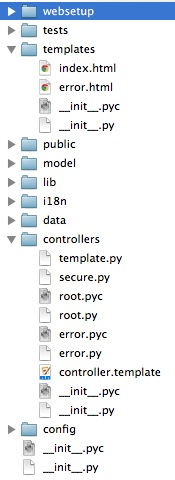
\includegraphics{img/tg2project.jpg}
\end{figure}

A seguire verranno descritte alcune delle cartelle più importanti.
\begin{description}
\item[model] contiene le classi necessarie a Ming per definire una struttura per i dati da salvare sul database.
\item[controllers] contiene i controller. \texttt{root.py} contiene tutte le funzioni di \emph{Piedmont Heritage}. \texttt{error.py} è creato da TG, si occupa della gestione degli errori.
\item[templates] contiene le pagine html del progetto.
\item[public] contiene tutte le risorse accessibili via web, come immagini, librerie javascript e fogli di stile.
\item[config e lib] contengono impostazioni e funzioni utili, utilizzate da TG e liberamente utilizzabili dal programmatore.
\end{description}

Il flusso di lavoro di TG potrebbe essere riassunto in:
\begin{enumerate}
\item Analizza l'url
\item Richiama l'opportuna funzione dell'opportuno controller
\item La funzione potrebbe interfacciarsi con il database, memorizzare o estrarre dati. 

In essa è sempre definito un \emph{decoratore}, il quale è una direttiva che indica alla View quale templare utilizzare. I dati da passare a Jinja devono essere memorizzati in un oggetto \texttt*dictionary* di python e restituiti dalla funzione. Un esempio è il listato \ref{ls:controller}, tratto dal root controller. La funzione si chiama \emph{detail}, come parametro ha la variabile ID passata secondo la modalità GET del protocollo HTTP. Essa viene richiamata nel caso in cui TG riceve una richiesta del tipo \texttt{hostname/detail\&id=unid}. \texttt{@expose} \`e il decoratore, in questo caso si richiede un output in formato json dei dati restituiti dalla funzione. Con questa funzione si interroga il database per ottenere informazioni su di un locale con ID=\emph{id}.
\item La view sostituisce i marker con le relative informazioni, infine genera la pagina
\item La pagina generata viene inviata al client che ha effettuato la richiesta.
\end{enumerate}

\begin{lstlisting}[label=ls:controller,caption={Esempio di funzione di un controller tratta dal root controller.},language=Python]
@expose('json')
def detail(self, id):
     det = c_locale.find({'_id': ObjectId(id)})
     return dict(data = list(det))
\end{lstlisting}

		
\subsection{Mongo DB}\label{sec:mongo}
Come spiegato nel capitolo \ref{sec:dbnonrel}, \emph{Mongo DB} è il DBMS utilizzato per il progetto, in cui vengono memorizzati i dati dei locali. Il sito del progetto è \url{www.mongodb.org}, in cui oltre al programma si può trovare il manuale ed un tutorial interattivo. Mongo come linguaggio di interrogazione non utilizza SQL a causa della sua natura NOSQL, ma utilizza javascript. Importantissimi sono il concetto di \emph{documento} e \emph{collezione}: in Mongo non esistono tabelle e relazioni, ma collezioni di documenti. Ogni documento è un oggetto javascript, che può contenere variabili liste e riferimenti ad altri oggetti, il tutto diviso per collezioni. Nel database vengono memorizzati gli oggetti Javascript tramite una funzione \texttt{save()}, ed è possibile estrarli utilizzando la funzione \texttt{find()}. Nel momento della creazione di un nuovo documento, Mongo aggiunge un campo \texttt{\_id} contenente un oggetto che rappresenta un identificativo univoco nella collezione, equivalente ad una chiave primaria di una tabella.

\section{Librerie}
\subsection{d3.js}\label{sec:d3}
D3.js è una libreria javascript che offre strumenti molto potenti per la visualizzazione di dati, il sito ufficiale è raggiungibile alla pagina \url{http://d3js.org/}. Oltre ad offrire funzioni per creare grafici utilizzando la \emph{Scalable Vector Graphics} di HTML\footnote{Più precisamente, il tag \texttt{svg}}, offre potenti strumenti di manipolazione di dati e di controllo del DOM.
		
\subsection{Polymaps}\label{sec:polymaps}
Polymaps (\url{http://polymaps.org/}) è una libreria javascript che utilizzando gli strumenti forniti da d3.js permette la creazione di mappe dinamiche, offrendo strumenti per effettuare operazioni su coordinate geospaziali. Sarà necessario ottenere le mappe in formato immagine da un server esterno, la libreria metterà quindi a disposizione strumenti come zoom e pan per spostarsi nella mappa.

			
\section{Funzionamento}%richiesta al server tramite url, AJAX per la richiesta dei dati, come opera turbogears, problemi e soluzioni
Piedmont Heritage è stato pensato in modo da dover caricare la pagina sul browser una sola volta, adottando quindi tecnologie che permettono la pagina di dialogare con il server in modo da permettere la . Quest'ultimo è quindi stato realizzato fornendo una funzione per il caricamento della pagina ed una serie di funzioni per il caricamento delle informazioni ottenute in modo autonomo dalla pagina.
\subsection{Lato client}
Solitamente quando un server web riceve una richiesta in cui la pagina non è specificata, controlla l'esistenza di un file chiamato \emph{index} e lo seleziona come risposta. Nel caso di Piedmont Heritage non è una pagina, ma una funzione chiamata \texttt{index}, riportata nel listato \ref{ls:index}. Il decoratore specificato indica il file \texttt{index.html} nella cartella \texttt{templates}. La natura ad oggetti del framework permette di considerare un oggetto anche una pagina web, in questo caso è stato utilizzato l'oggetto che lo rappresenta. La funzione si limita a restituire il titolo della pagina sotto forma di un dizionario di python, nel templare nel tag \texttt{<title>} è presente un segnaposto che verrà sostituito da questo valore.

\begin{lstlisting}[label=ls:index,caption={root controller, funzione index, richiamata alla richiesta della pagina web da parte del client.},language=Python]
@expose('pheritage.templates.index')
def index(self):
    """Handle the front-page."""
    return dict(page='index')
\end{lstlisting}

Una volta scaricata la pagina, al posto della mappa sarà presente un tag \texttt{svg} vuoto, che sarà completato dalla dalla chiamata a funzione \texttt{drawMap()} a fondo pagina\footnote{Una buona tecnica per evitare che il caricamento della pagina rimanga bloccato a causa del download degli script, è quello di spostare i tag \texttt{script} alla fine del documento.} che si occuperà di creare le strutture dati necessarie a mostrarla. 
\texttt{drawMap} è una funzione javascript definita nel file \texttt{public/js/map.js} che esegue queste operazioni:
\begin{enumerate}
\item seleziona nel DOM il tag \texttt{svg} prima citato
\item crea l'oggetto della mappa, settando la posizione nella pagina usando la variabile del punto 1, le coordinate geografiche a cui puntare e lo zoom.
\item assegna all'oggetto mappa la sorgente delle immagini raffiguranti la mappa vera e propria.
\item aggiungono i pulsanti per regolare lo zoom, per navigare nei risultati, ed il riquadro che visualizzerà i dettagli dei locali.
\item aggiunge l'oggetto mappa all'interno del tag \texttt{svg}, visualizzandolo effettivamente sulla mappa.
\end{enumerate}

I locali però non sono ancora stati caricati a questo punto, ma nemmeno le città ed i tipi selezionabili. La funzione \texttt{json()} di D3 ha la capacità di reperire dati in formato JSON dall'url passato come parametro. Il JSON, acronimo di JavaScript Object Notation, è un formato adatto per lo scambio dei dati in applicazioni client-server\footnote{cit. Wikipedia \url{http://it.wikipedia.org/wiki/JSON}} e consiste nel linguaggio utilizzato per definire oggetti in javascript. Tramite due chiamate alla funzione \texttt{json()} si reperiscono dal server l'elenco delle città e dei tipi, successivamente di inserisce ogni opzione nelle liste sopra la mappa.

Infine, si devono visualizzare i segnalini dei locali sulla mappa. La funzione \texttt{updateViz()} si occupa di controllare quali opzioni sono selezionate nei select delle città e dei tipi, ed effettuare una richiesta al server, tramite la funzione \texttt{json()} di D3. I risultati ottenuti rappresentano alla prima chiamata tutti i locali presenti del database, ed è necessario creare un puntino blu per ognuno di essi sulla mappa.

Come mostrato nel listato \ref{ls:enter} D3 dispone di una funzione chiamata \texttt{enter}, la quale permette effettuare operazioni per ogni elemento della lista. Per ogni elemento si visualizzerà un pallino creando un tag \texttt{circle}, dettando dimensione, colore e cosa deve accadere nel caso in cui si faccia click su di esso. Con \texttt{exit} si definiscono le operazioni da applicare agli elementi uscenti, ossia che non sono più nel risultato della ricerca e quindi non devono più essere presenti sulla mappa. Nel listato \ref{ls:enter} le istruzioni dopo \texttt{marker.exit()} dicono al programma di avviare un'animazione che porta la trasparenza a zero, facendoli svanire, per poi eliminare i tag \texttt{circle} dal DOM. Questo sistema di \emph{enter} ed \texttt{exit} è un'alternativa a scrivere un ciclo e permette di scrivere direttamente cosa deve fare D3 con ogni elemento.
\begin{lstlisting}[label=ls:enter,caption={\texttt{enter()} ed \texttt{exit()} di d3.js},language=c]
d3.json('points.json?city=' + settings.city + '&type=' + settings.type, function(points){
    selection.setData(points['data'])
    showDefaultDetails()
    // Add an svg:g for each station.
    var marker = layer.selectAll(".gcircle")
        .data(dat, function(d){
            //console.log(d)
            return d._id
            })
        
    marker.enter()
        .append("g")
        .on("click", selection.selectPoint)
        .attr('class', 'gcircle')
        .append("circle")
            .attr('class','circle')
            .attr("r", 3);
    
    marker.exit()
        .transition()
        .style('opacity', 0)        
        .duration(1000)
        .remove()
\end{lstlisting}

Viene poi mossa la mappa in modo che il punto \( (x, y) \) sia al centro, ricavato dalla funzione \ref{eq:centro} che calcola il punto medio tra i valori maggiore e minore di latitudine e longitudine. Infine si regola il focus in modo che tutti i punti siano visibili.
\begin{equation}
\label{eq:centro}
(x, y)=\left(\frac{max(lat)+min(lat)}{2}, \frac{max(lon)+min(lon)}{2}\right)
\end{equation}

A questo punto il programma aspetta input da parte dell'utente, e la mappa è interattiva. Grazie all'evento \texttt(move) polymaps rivela i drag del mouse sulla mappa, con il risultato di spostare la mappa ed i marker nella direzione dello spostamento del mouse. I tasti \texttt{+} e \texttt{-} in alto a sinistra permettono di modificare lo zoom, e cliccando su un marker verrà selezionato.
Quando un locale rappresentato da un punto viene selezionato, la funzione \texttt{seleciton} richiamata su di esso e viene mostrata un'animazione in cui la vecchia selezione torna un normale punto mentre quello nuovo cambia colore e si ingrandisce. D3 invia poi una richiesta al server contenente l'ID del locale e riceve le informazioni riguardanti il \emph{nome}, \emph{tipo}, \emph{periodo storico}, \emph{indirizzo} e \emph{comune}, e li visualizza nel box in alto a destra. 

Tramite un url che permette di ottenere un'immagine tratta da Google Street View che mostra una visuale di un certo indirizzo, viene mostrato il luogo che secondo Google Maps corrisponde all'indirizzo memorizzato. Questa feature è stata inserita sperimentalmente, ma non offre una panoramica soddisfacente del posto e non tutti gli indirizzi hanno un'immagine associata.

\`E possibile selezionare i locali uno per uno, utilizzando i pulsanti di navigazione in alto al centro. La pressione di quei pulsanti non farà altro che aumentare o diminuire l'iterator che punta all'oggetto selezionato nella lista dei risultati e richiamare la funzione \texttt{selection} su di esso.

L'ultima funzionalità è quella della ricerca per comune e/o tipo. Selezionando un elemento nel menu \texttt{select} dei comuni la lista dei tipi viene modificata mostrando solo i tipi disponibili in quel comune, sempre grazie a d3 ed una funzione scritta nel server. Premendo il tasto \emph{filtra}, verrà richiesto al server l'elenco di locali che soddisfano i criteri selezionati, e si affideranno i risultati a d3, il quale provvederà a visualizzare i nuovi punti ed eliminando quelli non più presenti come descritto in precedenza.

\subsection{Lato server}









\end{document} 